\documentclass{article}
\usepackage{multicol}
\usepackage{hyperref}
\usepackage{geometry}
\usepackage[sorting=none]{biblatex}
\usepackage{titlesec}
\usepackage{float}
\usepackage{amsmath}
\usepackage{amssymb}
\usepackage{graphicx}
\usepackage{tikz}
\usepackage{booktabs}
\usepackage{siunitx}
\usepackage{mathtools}
\usepackage[linesnumbered,ruled,vlined]{algorithm2e}
% \usepackage{bbm}
\usepackage{setspace}

\addbibresource{references.bib}
\numberwithin{figure}{section}
\numberwithin{table}{section}
\numberwithin{equation}{section}
\geometry{margin=0.9in}
% \titleformat{\section}{\large\bfseries\scshape}{\thesection}{1em}{}
% \titleformat{\subsection}{\normalfont\bfseries\scshape}{\thesubsection}{1em}{}
% \titleformat{\subsubsection}{\small\bfseries\scshape}{\thesubsubsection}{1em}{}

\title{\large Course of Control Problems in Robotics \\ \LARGE Control of underactuated robots via input-constrained receding-horizon differential dynamic programming}
\author{Simone Orelli\\1749732 
\and Antonio Rapuano\\2044902
\and Dhaval Shukla \\2047562 \and \textit{DIAG Department}\\ \textit{University of Rome “La Sapienza”}\\ $[$surname$]$.$[$id number$]$@studenti.uniroma1.it}
\date{October 2024}

\begin{document}
    \maketitle
    \thispagestyle{empty}
        \begin{multicols}{2}
            \vfill\null\null
        \begin{abstract}
    This paper details the process of developing a control system for Ingenuity, a drone helicopter that operated from 2021 to 2024 on Mars as part of NASA's Mars 2020 mission. Said process consists first of creating a mathematical model capable of representing the behavior of the drone in flight over Mars, and then designing a controller capable of imparting desired behavior and performance (trajectory tracking) to the model. 
    The problem is approached through two different control strategies: first, with a static input-to-output feedback linearization controller, and then, through the backstepping technique. Among the two, only the latter returns satisfactory results, as it is able to achieve the objectives by exploiting the fact that Ingenuity is an underactuated robot.
\end{abstract}
        \vfill\null
        \columnbreak
        \tableofcontents

        \newpage
        \pagenumbering{arabic}
        \section{Introduction}
In NASA's Mars 2020 mission, the helicopter \textit{Ingenuity} was deployed to demonstrate the first powered flight on another planet. The helicopter was designed to be a technology demonstrator, and its main goal was to prove that powered flight in the thin Martian atmosphere is possible. By the date of the end of its mission (caused by the rupture of one of the rotor blades), Ingenuity had far exceeded every expectation: originally designed to perform up to five experimental test flights over 30 days, instead it flew for almost three years, performing 72 flights, and traversing more than 14 times the planned distance.

In the upcoming sections of the document we will present a mathematical model of Ingenuity, and we will discuss the control strategies that can be used to stabilize and control it, possibly around a planned trajectory, during flight in the Martian atmosphere. The theoretical results will be validated through simulated experiments.

\subsection{Helicopter structure}
At its core, Ingenuity features a fuselage designed for minimal weight and maximum strength, a sturdy framework for housing critical components such as the avionics, power system, and rotor assembly.

The most prominent feature is its coaxial rotor system, comprising two horizontally-overlapping counter-rotating (to mitigate reaction torque effects) blades, ensuring stability and precise maneuverability during flight. Attached to the rotor system is a central mast, which extends upward from the fuselage.

\begin{figure}[H]
    \centering
    \includegraphics[width=0.7\columnwidth]{figures/ingenuity_render.png}
    \caption{3D render of the Ingenuity Mars Helicopter.}
    \label{fig:ingenuity_render}
\end{figure}

Complementing these is a suite of sensors, cameras, and communication equipment strategically integrated throughout Ingenuity's structure. These instruments enable it to navigate autonomously according to the instructions coming from the base of operation on Earth and capture imagery of the Martian surface.

The main parameters of the helicopter structure model are summarized in Table \ref{tab:ingenuity_parameters}.

\begin{table}[H]
    \centering
    \begin{tabular}{|c|c|c|}
        \hline
        \textbf{Parameter} & \textbf{Symbol} & \textbf{Value} \\
        \hline
        \hline
        Mass & $m$ & \SI{1.8}{\kilogram} \\
        \hline
        Rotor diameter & $2\,r$ & \SI{1.2}{\meter} \\
        \hline
        Blade chord & $c$ & \SI{0.24}{\meter} \\
        \hline
        \begin{tabular}{@{}c@{}}COM - upper\\rotor distance\end{tabular} & $d_{cm, u}$ & \SI{0.10}{\meter} \\
        \hline
        \begin{tabular}{@{}c@{}}COM - lower\\rotor distance\end{tabular} & $d_{cm, l}$ & \SI{0.05}{\meter} \\
        \hline
        Inertia & $I$ & \begin{tabular}{@{}c@{}}$diag(0.210, 0.288, $\\$0.278)$\,\SI{}{\kilogram\square\meter}\end{tabular} \\
        \hline
    \end{tabular}
    \caption{Structural parameters of the Ingenuity model.}
    \label{tab:ingenuity_parameters}
\end{table}

\subsection{Martian environment}
Even though the Martian gravity is only about $38\%$ of the Earth's, its thin atmosphere, composed mainly of carbon dioxide with a ground-level pressure of about $0.6\%$ of the Earth's, makes it difficult for aerial vehicles to fly. The athmospheric model is split in two zones: below and above the altitude of $\SI{7000}{\meter}$. Since Ingenuity only performs low level flights, we are interested in the parameters of the lower layer, whose expressions (with respect to altitude) are summarized in Table \ref{tab:martian_environment}.

\begin{table}[H]
    \centering
    \begin{tabular}{|c|c|c|}
        \hline
        \textbf{Parameter} & \textbf{Sym} & \textbf{Value} \\
        \hline
        \hline
        Gravity & $g$ & \SI{3.71}{\meter\per\square\second} \\
        \hline
        Temperature & $T$ & $-242.1-9.98 \times 10^{-4} \, h$\;\SI{}{\kelvin} \\
        \hline
        Pressure & $p$ & $0.699 \, e^{-0.9 \times 10^{-5} h}$\;\SI{}{\kilo\pascal} \\
        \hline
        Air density & $\rho$ & $p/(0.192\;T)$\;\SI{}{\kilogram\per\cubic\meter} \\
        \hline
    \end{tabular}
    \caption{Martian environment parameters for altitude $h< \SI{7000}{\meter}$.}
    \label{tab:martian_environment}
\end{table}


        \section{Differential dynamic programming}
This section provides a brief overview of the Differential Dynamic Programming (DDP) algorithm. Part of what follows is reprised and recast mostly from \cite{tassa07}.

\subsection{Optimal control problem}
The numerical implementation of the DDP algorithm is constructed on a time-discrete optimal control problem that encodes both the dynamics of the system and the control objective.

One possible way for the mathematical model to be discretized is to use the well-known forward Euler method. \\
Given a state vector $x$, a control input $u$, and the time step $T$, the discretized dynamics are given by:
\begin{equation}
    x^{i+1} = F(x^i, u^i) = x^i + T f(x^i, u^i), \label{eq:dyn}
\end{equation}
where $f(x, u)$ is the continuous-time dynamics of the system.

The cost function to minimize comes from the sum of the running cost $l(x, u)$ and the terminal cost $l_f(x)$. Simple and common choices for these functions are quadratic forms.\\
Accordingly to \ref{eq:dyn}, over a control horizon of duration $N$, the state sequence $X = {\{x^i\}_{i=0}^{N}}$ is uniquely identified by the initial state $x^0$ and the control sequence $U = {\{u^i\}_{i=0}^{N-1}}$. Therefore, the total cost is given by:
\begin{equation}
    J(x^0, U) = \sum_{i=0}^{N-1} l(x^i, u^i) + l_f(x^N) \label{eq:cost}
\end{equation}

In light of the above, the optimal control problem we will be solving is the following.
\begin{equation*}
    \begin{aligned}
        \min_U & \quad J(x^0, U) = \sum_{i=0}^{N-1} l(x^i, u^i) + l_f(x^N) \\
        \text{s.t.} & \quad x^{i+1} = F(x^i, u^i), \quad \;\; i = 0, \ldots, N-1
    \end{aligned}
\end{equation*}
where the optimal control sequence $U^*$ is the one to feed to the system.\\
Notice that the DDP algorithm alone does not allow to enforce a constraint on the final state, meaning that the terminal cost is crucial to guide the system towards the desired equilibrium.

\subsection{Local dynamic programming}
The DDP algorithm plays around the so-called \textit{value} function, defined as the minimum cost-to-go from time $i$ to the end of the horizon:
\begin{equation*}
    V^i(x^i) = \min_{U^i} \left\{ \sum_{j=i}^{N-1} l(x^j, u^j) + l_f(x^N) \right\},
\end{equation*}
where $U^i = \{u^j\}_{j=i}^{N-1}$ is the control sequence from time $i$ to the end of the horizon. In particular:
\begin{equation}
    V^N(x^N) = l_f(x^N). \label{eq:vf_N}
\end{equation}
According to Bellman's principle of optimality \cite{bellman} and using \ref{eq:dyn}, the value function can be rewritten as\footnote{For the sake of brevity, we henceforth omit the time index $i$ and denote by $V^\prime$ the value referring to the next instant $i+1$.}:
\begin{equation*}
    V(x) = \min_{u} \left\{ l(x, u) + V^\prime(F(x, u)) \right\}.
\end{equation*}
We call \textit{Q-function} the minimization argument:
\begin{equation}
    Q(x, u) = l(x, u) + V^\prime(F(x, u)), \label{eq:qfun}
\end{equation}
leading to:
\begin{equation}
    V(x) = \min_{u} Q(x, u). \label{eq:vfun}
\end{equation}

\subsection{Quadratic approximation}
If we consider a nominal state-control pair $(\overline{x}, \overline{u})$, the Q-function can be approximated by a second-order Taylor expansion around these:
\begin{gather}\label{eq:qfun_taylor}
    Q(\overline{x}+\delta x, \overline{u}+\delta u) \approx Q(\overline{x}, \overline{u}) + Q_x^\top(\overline{x}, \overline{u}) \delta x\;+ \nonumber \\
    +\;Q_u^\top(\overline{x}, \overline{u}) \delta u + \frac{1}{2} \begin{bmatrix} \delta x \\ \delta u \end{bmatrix}^\top \begin{bmatrix}Q_{xx} & Q_{xu} \\ Q_{ux}  & Q_{uu} \end{bmatrix}(\overline{x}, \overline{u}) \begin{bmatrix} \delta x \\ \delta u \end{bmatrix}.
\end{gather}
The values of the gradient and Hessian of the Q-function can be computed by expanding also \ref{eq:qfun} and equating the coefficients of the same order. Therefore, we get\footnote{Once again for brevity, we neglect the dependence on the nominal state-control pair $(\overline{x}, \overline{u})$.}:
\begin{align}
    Q_x &= l_x + V^{\prime\top}_x F_x, \label{eq:qx} \\ 
    Q_u &= l_u + V^{\prime\top}_x F_u, \\
    Q_{xx} &= l_{xx} + F_x^\top V^\prime_{xx} F_x + V^\prime_x F_{xx},\\
    Q_{uu} &= l_{uu} + F_u^\top V^\prime_{xx} F_u + V^\prime_x F_{uu},\\
    Q_{xu} &= l_{xu} + F_x^\top V^\prime_{xx} F_u + V^\prime_x F_{xu}. \label{eq:qxu}
\end{align}
The optimal control adjustment in response to a state deviation $\delta x$ is obtained by minimizing the Q-function with respect to $\delta u$, yielding the local state-affine policy:
\begin{equation}
    \delta u^\star = k + K \delta x, \label{eq:deltau_star}
\end{equation}
with coefficients given by:
\begin{align}
    k &= -Q_{uu}^{-1} Q_u, \label{eq:k} \\ 
    K &= -Q_{uu}^{-1} Q_{ux}. \label{eq:K}
\end{align}
Similarly, the we can also expand the value function:
\begin{equation*}
    V(\overline{x} + \delta x) \approx V(\overline{x}) + V_x^\top(\overline{x}) \delta x + \frac{1}{2} \delta x^\top V_{xx}(\overline{x}) \delta x.
\end{equation*}
Using \ref{eq:vfun} with $x = \overline{x}+ \delta x$ and $u = \overline{u} + \delta u$, and plugging \ref{eq:deltau_star} into \ref{eq:qfun_taylor}, we can extract the gradient and Hessian of the value function, whose expressions, once simplified according to \cite{tassa12}, are:
\begin{align}
    V_x &= Q_x - K^\top Q_{uu} k,\label{eq:vx} \\ 
    V_{xx} &= Q_{xx} - K^\top Q_{uu} K. \label{eq:vxx}
\end{align}

\subsection{Backward and forward sweeps}
Given an initial control sequence $U_{\text{init}}$, the first real step of the algorithm is to compute the corresponding state evolution $X_{\text{init}}$ by recursively applying \ref{eq:dyn}.\\
We can consider these as the nominal trajectories, making it possible to compute $V^N(\overline{x}^N)$ according to \ref{eq:vf_N}, which unlocks the ability to calculate the coefficients of the expansion of the Q-function around the pair $(\overline{x}^{N-1}, \overline{u}^{N-1})$ using \ref{eq:qx} - \ref{eq:qxu}. These form the gains $k$ in \ref{eq:k} and $K$ in \ref{eq:K}, which in turn allow us to find the coefficients of the expansion of the value function $V(\cdot)$ around $(\overline{x}^{N-1}, \overline{u}^{N-1})$ with \ref{eq:vx} and \ref{eq:vxx}, and so on until the initial state $x^0$ is reached. This phase is called the \textit{backward sweep}.\\
Subsequently, the \textit{forward sweep} consists of recursively applying the local state-affine policy \ref{eq:deltau_star} to the state deviation $\delta x^i = x^i - \overline{x}^i$, exploiting once again \ref{eq:dyn} to obtain new control and state sequences from the previous (nominal) ones using:
\begin{align}
    x^0 &= \overline{x}^0, \label{eq:x0} \\
    u^i &= \overline{u}^i + k^i + K^i (x^i - \overline{x}^i). \label{eq:u_update}
\end{align}
The alternation of backward and forward sweeps goes on until a satisfactory solution is found.

\subsection{Regularization}
In this part, we focus on common weaknesses of DDP and how they can be addressed in the implementation phase.

\subsubsection{Levenberg-Marquardt parameter}
The Hessian of the Q-function $Q_{uu}$ is required to be positive definite in order to guarantee the existence of a minimum. To ensure this, a regularization term is added, and the resulting modified Hessian $\tilde{Q}_{uu}$ is then used to compute the gains $k$ and $K$. The regularization term is proportional to the identity matrix and is weighted by a scalar $\mu$, that plays the role of a Levenberg-Marquardt parameter:
\begin{equation}
    \tilde{Q}_{uu} = Q_{uu} + \mu I. \label{eq:q_uu_reg}
\end{equation}
This corresponds to adding a quadratic term around the current control sequence, which makes the steps more conservative. \\
Further details can be found in \cite{tassa12}.

\subsubsection{Line search}
At each forward sweep, an issue may arise if the newly found trajectory significantly diverges from the previous one, resulting in a substantial error in the quadratic approximation. To prevent this, a line search is performed to find the optimal step size $\alpha$ that minimizes the cost along the direction of the control adjustment. This is done by iteratively reducing (usually halving) the step size until the cost of the proposed trajectory decreases sufficiently (i.e., it becomes smaller than the cost of the nominal one), and then performing the step. Logically, if $\alpha$ becomes too small it means that the optimal trajectory has been found.\\
The implementation of the line search is done by integrating $\alpha$ in the forward sweep, so that the control sequence is updated as:
\begin{equation}
    u^i = \overline{u}^i + \alpha k^i + K^i (x^i - \overline{x}^i), \label{eq:u_update_alpha}
\end{equation}
indeed replacing \ref{eq:u_update}. Notice that the feedback term is not affected by the line search.

        \section{Optimal controller}
The aim of this section is to design an optimal control law that exploits the DDP algorithm in such a way that a nonlinear system (such as a robot) is led to an objective optimally with respect to some cost. 

\subsection{Hard input constraints}
Within the robotics field, actuators are often subject to saturation limits. In the case of revolute joints, the torque that can be applied is limited by the maximum torque that the motor can supply. The presence of these limitations translates into the birth of hard constraints on the input of the form of \ref{eq:input_constraints}, referred to as \textit{box constraints}. \\
We propose three alternatives derived from \cite{tassa14} to handle these constraints.

\subsubsection{Naive clamping}
A simple way to handle the constraints is to clamp the control input in the forward sweep to the limits of the box constraints. The operation performed element-wise on the control input vector $u$ is:
\begin{equation*}
    \mathcal{N}\mathcal{C}(u) =\min\{\max\{u, u_{\text{min}}\}, u_{\text{max}}\}.
\end{equation*}
As a consequence, \ref{eq:u_update_alpha} becomes:
\begin{equation}
    u^i = \mathcal{N}\mathcal{C}(\overline{u}^i + \alpha k^i + K^i (x^i - \overline{x}^i)). \label{eq:u_update_alpha_clamp}
\end{equation} 
The drawback of such a trivial intervention is that the clamped search direction may not be feasible anymore, compromising convergence.

\subsubsection{Squashing functions}
Another way to enforce the constraints is to use component-wise sigmoidal squashing functions, such as the following.

\begin{equation*}
    \mathcal{S}(u) = \frac{u_{\text{max}} - u_{\text{min}}}{2} \tanh\frac{2\,u}{u_{\text{max}} - u_{\text{min}}} + \frac{u_{\text{max}} + u_{\text{min}}}{2},
\end{equation*}
where the hyperbolic tangent is used to squash the input to the interval $[u_{\text{min}}, u_{\text{max}}]$:
\begin{equation*}
    \lim_{u \to -\infty} \mathcal{S}(u) = u_{\text{min}}, \quad \lim_{u \to +\infty} \mathcal{S}(u) = u_{\text{max}}.
\end{equation*}
Correspondigly, the update rule for the control input \ref{eq:u_update_alpha} becomes:
\begin{equation}
    u^i = \mathcal{S}(\overline{u}^i + \alpha k^i + K^i (x^i - \overline{x}^i)). \label{eq:u_update_alpha_squash}
\end{equation}
In the cost function, the unmodified control inputs should be used in order to prevent their explosion. 
Altough the squashing function is differentiable, its nonlinearity is not well captured by the quadratic approximation of the dynamics that is being performed in the backward pass. This may lead to suboptimal solutions or even convergence issues.

\subsubsection{Constrained quadratic programming}
The best-performing method to take into account the control limitations is to condition, through the constraints, the minimization of the quadratic model of the Q-function.\\
At the moment, the solution \ref{eq:deltau_star} is valid in the unconstrained case. To include the constraints, the idea is to solve the following constrained quadratic program:
\begin{equation*}
    \begin{aligned}
        \min_{\delta u} \quad & Q(\overline{x} + \delta x, \overline{u} + \delta u) \\
        \text{s.t.} \quad & u_{\text{min}} \leq \overline{u} + \delta u \leq u_{\text{max}}.
    \end{aligned}
\end{equation*}
With reference to \ref{eq:qfun_taylor}, we know that the minimization argument depends both on $\delta x$ and $\delta u$. Being $\delta u$ the minimization variable, since $\delta x$ is unknown during the backward sweep, a direct solution can be found only for the feedforward term:
\begin{equation}
    \begin{aligned}
        k = \text{arg}\min_{\delta u} & \left\{Q_u ^\top \delta u + \frac{1}{2} \delta u^\top Q_{uu} \delta u \right\}\\
        \text{s.t.} \;& \;\,u_{\text{min}} \leq \overline{u} + \delta u \leq u_{\text{max}},
    \end{aligned} \label{eq:k_qp}
\end{equation}
which replaces \ref{eq:k}.\\
In order to find the feedback term $K$, the Hessian $Q_{uu}$ must be decomposed as $Q_{uu} = Q_{uu}^f + Q_{uu}^c$, where $Q_{uu}^f$ is the submatrix corresponding to the free dimensions of the control input, and $Q_{uu}^c$ is the submatrix corresponding to the clamped dimensions. Then, instead of \ref{eq:K}, the feedback term is computed as:
\begin{equation}
    K = -Q_{uu}^f Q_{ux}, \label{eq:K_qp}
\end{equation} 
implying that the rows of $K$ corresponding to clamped controls are identically zero.\\
In addition, we have found that applying the naive clamping on top of this in the forward sweep ensures the feasibility of the input even in the event that, despite the control dimension falling within the free section of $Q_{uu}$, the action of the feedback term on the state deviation causes the control to exceed its boundaries.

\subsection{Receding-horizon control}
Following the proposed scheme, the DDP algorithm can certainly identify an optimal control sequence that, combined with the nominal dynamics of the system, returns a state evolution that satisfies a high-level objective. In order to design a control law inducing the system to perform its intended task with robustness guarantees with respect to model uncertainty and possible presence of disturbances, we propose to enrich the algorithm with a receding horizon control logic, in the spirit of Model Predictive Control (MPC).

Briefly, the idea is to apply the DDP algorithm at each time step, considering the current state as the initial state, and the current control sequence as the initial guess. The first control input of the optimal sequence is then applied to the system, and the process is repeated at the next time step. This way, the control law is updated at each time step, and the system is driven to the desired state in a receding horizon fashion.\\
To this end, crucial is the computation of the very first control sequence, which should be carried out employing enough resources to identify an optimal (or close to the optimal) trajectory. The following iterations, on the other hand, can be performed with less computational effort, since the algorithm is already warm-started with a good initial guess, therefore allowing for real-time applications.

\subsection{Implementation}
We investigate the implementation of the control algorithm in the following pseudocode. The algorithm is composed of four main functions, respectively implementing the backward sweep, the forward sweep, one single iteration of the DDP algorithm and the whole receding-horizon controller. 

\begin{figure}[H]
    \centering
    \begin{algorithm}[H]
        \caption{Backward sweep (\textit{bwd})}
        \label{alg:bwd}
        \setstretch{1.1}
        \KwData{$x^0$, $U = \{u^i\}_{i=0}^{N-1}$}
        \KwResult{$G = \{(k^i, K^i)\}_{i=0}^{N-1}$}

        Compute $X = \{x^i\}_{i=0}^{N}$ by applying recursively \ref{eq:dyn} to $x^0$ with $U$\;
        Compute $V^\prime_x = l_{f, x}(x^N)$ and $V^\prime_{xx} = l_{f, xx}(x^N)$ according to \ref{eq:vf_N}\;

        \For{$i = N-1, \dots, 0$} {
            Compute $Q_u$, $Q_x$, $Q_{xx}$, $Q_{uu}$ and $Q_{xu}$ using \ref{eq:qx} - \ref{eq:qxu}\;
            If necessary, regularize $Q_{uu}$ using \ref{eq:q_uu_reg}\;
            Compute $k^i$ and $K^i$ using \ref{eq:k_qp} and \ref{eq:K_qp}\;
            Compute $V_x$ and $V_{xx}$ using \ref{eq:vx} and \ref{eq:vxx}\;
            Set $V'_x = V_x$ and $V'_{xx} = V_{xx}$\;
        }
    \end{algorithm}
\end{figure}

Starting from an initial state $x^0$ and a control sequence $U$, Algorithm \ref{alg:bwd} realizes the function \textit{bwd}, which computes the gain sequence $G = \{(k^i, K^i)\}_{i=0}^{N-1}$ by iteratively applying the constrained quadratic programming.

Given a nominal trajectory and a sequence of gains, Algorithm \ref{alg:fwd} implements a function named \textit{fwd}, which iteratively computes the modified trajectory by applying the constrained local state-affine policy $\delta u^\star$ to the state deviation, using $\alpha$ as a step-size for the feedforward term.

\begin{figure}[H]
    \centering
    \begin{algorithm}[H]
        \caption{Forward sweep (\textit{fwd})}
        \label{alg:fwd}
        \setstretch{1.1}
        \KwData{$x^0$, $\overline{U} = \{\overline{u}^i\}_{i=0}^{N-1}$, $G = \{(k^i, K^i)\}_{i=0}^{N-1}$, $\alpha$}
        \KwResult{$U = \{u^i\}_{i=0}^{N-1}$}

        Compute $\overline{X} = \{\overline{x}^i\}_{i=0}^{N}$ by applying recursively \ref{eq:dyn} to $\overline{x}^0 = x^0$ with $\overline{U}$\;

        \For{$i = 0, \dots, N-1$} {
            Compute $u^i$ using \ref{eq:u_update_alpha}\;
            Constrain $u^i$ using \ref{eq:u_update_alpha_clamp} or \ref{eq:u_update_alpha_squash}\;
            Compute $x^{i+1}$ using \ref{eq:dyn}\;
        }
    \end{algorithm}
\end{figure}

Algorithm \ref{alg:ddp} realizes the application of an iteration of DDP, alternating between backward and forward sweeps until the cost converges to a minimum. Moreover, this function executes the line search to find the step size $\alpha$ that leads to a decrease in the cost. If the cost does not decrease, being stuck in the loop signifies that we are already at the minimum, therefore the algorithm stops.

\begin{figure}[H]
    \centering
    \begin{algorithm}[H]
        \caption{DDP iteration (\textit{ddp})}
        \label{alg:ddp}
        \setstretch{1.1}
        \KwData{$x^0$, $U_{\text{init}} = \{u_{\text{init}}^i\}_{i=0}^{N-1}$}
        \KwResult{$U^\star = \{u^{\star,i}\}_{i=0}^{N-1}$}
        Initialize $U = U_{\text{init}}$\;
    
        \Repeat{$\alpha \approx 0$} {
            Compute the cost $J$ using \ref{eq:cost}\;
            Perform a backward sweep $G = \textit{bwd}(x^0, U)$\;
    
            Reset $\alpha$\;
            \Repeat{$\alpha \approx 0 \lor J' < J$}{
                Perform a forward sweep $U^\prime = \textit{fwd}(x^0, U, G, \alpha)$\;
                Compute the cost $J^\prime$ using \ref{eq:cost} with $U^\prime$\;
                Halve $\alpha$\;
            }
            Set $U = U^\prime$\;
        }
        Set $U^\star = U$\;
    \end{algorithm}
\end{figure}

Finally, Algorithm \ref{alg:rh} implements the previously-discussed receding-horizon control logic. Its purpose is to iteratively apply the DDP algorithm to the system, identifying the best the control input at each time step in function of on-line measurements of the state.

\begin{figure}[H]
    \centering
    \begin{algorithm}[H]
        \caption{Receding-horizon control}
        \label{alg:rh}
        \setstretch{1.1}
        Initialize $U_{\text{init}} = \{0\}_{i=0}^{N-1}$\;

        \Repeat{termination condition} {
            Measure the current state $x$\;
            Perform a DDP iteration $U^\star = \textit{ddp}(x, U_{\text{init}})$\;
            Apply the first control input $u^{\star,0}$ to the system\;
            Set $U_{\text{init}} = \{u^{\star,i}\}_{i=1}^{N-1}$\;
            Append $\{u^{\star,N}\}$ to $U_{\text{init}}$\;
        }
    \end{algorithm}
\end{figure}
        \section{Control of underactuated robots}
The present section delves into the application of the strategy illustrated so far to the control of two examples of underactuated robots - the pendubot and the acrobot.
\subsection{Mathematical model}
The pendubot and the acrobot share the same dynamics of a 2R planar robot moving in the vertical plane. With reference to \cite{lanarioriolo}, which in turn quotes \cite{siciliano}, to describe these dynamics we introduce the system of differential equations:
\begin{equation}
    M(q) \ddot{q} + B \dot{q} + c(q, \dot{q}) + e(q) = u, \label{eq:dyn_robot}
\end{equation}
where $q = \begin{bmatrix} q_1 & q_2 \end{bmatrix}^\top$ is the vector of joint angles, $\dot{q}$ and $\ddot{q}$ are the joint velocity and acceleration, respectively, and $u = \begin{bmatrix} u_1 & u_2 \end{bmatrix}^\top$ is the control input. \\
Moreover, $M(q)$ is the inertia matrix:
\begin{equation*}
    M(q) = \begin{bmatrix}
        a_1 + 2a_2 c_2 & a_3 + a_2 c_2 \\
        a_3 + a_2 c_2 & a_3
    \end{bmatrix},
\end{equation*}
$B$ is the (positive definite) dissipation matrix: 
\begin{equation*}
    B = \begin{bmatrix}
        b_1 & 0 \\
        0 & b_2
    \end{bmatrix},
\end{equation*}
$c(q, \dot{q})$ is the Coriolis and centrifugal vector: 
\begin{equation*}
    c(q, \dot{q}) = \begin{bmatrix}
        a_2 s_2 \dot{q}_2 (\dot{q}_2 + 2 \dot{q}_1) \\
        a_2 s_2 \dot{q}_1^2
    \end{bmatrix},
\end{equation*}
and $e(q)$ is the gravity vector:
\begin{equation*}
    e(q) = \begin{bmatrix}
        a_4 s_1 + a_5 s_{12} \\
        a_5 s_{12}
    \end{bmatrix}.
\end{equation*}
Here, we use the compact notation:
\begin{align*}
    s_1 &= \sin(q_1), & c_1 &= \cos(q_1), \\
    s_2 &= \sin(q_2), & c_2 &= \cos(q_2), \\
    s_{12} &= \sin(q_1 + q_2), & c_{12} &= \cos(q_1 + q_2),
\end{align*}
and the (positive) constants:
\begin{align*}
    a_1 &= I_{1zz} + m_1 d_1^2 + I_{2zz} + m_2 (l_1^2 + d_2^2), \\
    a_2 &= m_2 l_1 d_2, \\
    a_3 &= I_{2zz} + m_2 d_2^2, \\
    a_4 &= g (m_1 d_1 + m_2 l_1), \\
    a_5 &= g m_2 d_2.
\end{align*}
\begin{figure}[H]
    \centering
    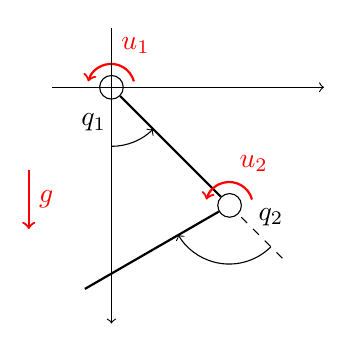
\begin{tikzpicture}[scale=1.5]
        \coordinate (O) at (0,0);
        \coordinate (A) at (1,-1);
        \coordinate (B) at (-0.225,-1.707);
        \coordinate (C) at (1.48,-1.48);
        
        \draw[thick] (O) -- (A) -- (B);
        \draw[dashed] (A) -- (C);
        
        \filldraw[white] (O) circle (0.1);
        \draw (O) circle (0.1);
        \filldraw[white] (A) circle (0.1);
        \draw (A) circle (0.1);
        
        \draw[->] (0,-0.5) arc[start angle=270, end angle=315, radius=0.5];
        \draw[->] (A) ++(0.35,-0.35) arc[start angle=315, end angle=210, radius=0.5];
        
        \node at (-0.15,-0.3) {$q_1$};
        \node at (1.35,-1.1) {$q_2$};
        
        \draw[red,->,thick] (O) ++(0.19,0.05) arc[start angle=15, end angle=165, radius=0.2] node[midway, above right] {$u_1$};
        \draw[red,->,thick] (A) ++(0.19,0.05) arc[start angle=15, end angle=165, radius=0.2] node[midway, above right] {$u_2$};
        
        \draw[red,->,thick] (-0.7,-0.7) -- ++(0,-0.5) node[midway, right] {$g$};
        
        \draw[->] (-0.5,0) -- (1.8,0);
        \draw[->] (0,0.5) -- (0,-2);
    \end{tikzpicture}
    \caption{Graphical representation of a 2R planar robot in the vertical plane.}
    \label{fig:robot}
\end{figure}
The only difference between the two robots lies in the actuation, since the only actuated joint of the pendubot is the “shoulder” (implying that $u_2 = 0$), while that of the acrobot is the “elbow”(therefore $u_1 = 0$).

\subsection{Control objective}
The equilibria of the robot are found by setting all the derivatives of the generalized coordinates to zero. Among these, the unforced ones are identified by solving the equation:
\begin{equation*}
    e(q) = 0,
\end{equation*}
which corresponds to the condition of balance of the gravity forces, yielding the four solutions:
\begin{equation*}
    q_{uu} = \begin{bmatrix} \pi \\ 0 \end{bmatrix}, \quad
    q_{ud} = \begin{bmatrix} \pi \\ \pi \end{bmatrix}, \quad
    q_{du} = \begin{bmatrix} 0 \\ \pi \end{bmatrix}, \quad
    q_{dd} = \begin{bmatrix} 0 \\ 0 \end{bmatrix}.
\end{equation*}

The control objective is to stabilize the robot in the upright position $q_{uu}$ with zero final velocity, starting from the initial conditions $q_0 = q_{dd}$ and $\dot{q}_0 = 0$. This is known as the \textit{swing-up problem}, and it is a challenging task due to the underactuation of the system, since the control input is constrained to the actuated joint, and the other joint is passive.

In addition, the control input is subject to the (component-wise) inequality constraint:
\begin{equation}
    u_{\text{min}} \leq u \leq u_{\text{max}}, \label{eq:input_constraints}
\end{equation}
to be intended as a saturation limit on the torque that can be applied to the actuated joint. Obviously, the input is also subject to the physical constraint $u_2 = 0$ for the pendubot and $u_1 = 0$ for the acrobot, and therefore $u_{\text{min}}$ must be non-positive and $u_{\text{max}}$ non-negative.

\subsection{Control strategy tailoring}
The control strategy illustrated so far can be adapted to the specific case of the pendubot and the acrobot by considering the following. 

\subsubsection{Dynamics}
First of all, we have to translate our nonlinear dynamics \ref{eq:dyn_robot} in terms of \ref{eq:dyn}. To this end, we define the state vector: 
\begin{equation*}
    x = \begin{bmatrix} x_1 & x_2 & x_3 & x_4 \end{bmatrix}^\top = \begin{bmatrix} q^\top & \dot{q}^\top \end{bmatrix}^\top.
\end{equation*}
As far as the control input is concerned, we use: 
\begin{equation*}
    u = \begin{bmatrix} u_1 & 0 \end{bmatrix}^\top
\end{equation*}
for the pendubot and: 
\begin{equation*}
    u = \begin{bmatrix} 0 & u_2 \end{bmatrix}^\top
\end{equation*}
for the acrobot. Therefore, the dynamics of the robot, rewritten in terms of \ref{eq:dyn}, are given by defining the $4\times1$ state transition function:
\begin{equation*}
    f(x, u) = \begin{bmatrix} x_3 \\ x_4 \\ M^{-1}(x)\left(-B\begin{bmatrix}x_3 \\ x_4\end{bmatrix} - c(x) - e(x) + u\right) \end{bmatrix}.
\end{equation*}

Finally, according to this new representation, the swing-up problem undergoes the following modifications:
\begin{itemize}
    \item the initial state is $x_0 = \begin{bmatrix} q_{dd}^\top & 0 & 0 \end{bmatrix}^\top$;
    \item the (final) reference state is $x^* = \begin{bmatrix} q_{uu}^\top & 0 & 0 \end{bmatrix}^\top$.
\end{itemize}

\subsubsection{Cost function}
Another important object to tailor is the cost function \ref{eq:cost}, and, for this purpose, a common and simple choice is to use quadratic functons. In particular, we select:
\begin{align*}
    l(x,u) &= (x-x^*)^\top P (x-x^*) + u^\top R u,\\
    l_f(x) &= (x-x^*)^\top P^N (x-x^*),
\end{align*}
where $P$, $R$ and $P^N$ are positive definite matrices. The choice of the cost function is fundamental, since it determines the behavior of the control law. In this case, in the spirit of our control objective, we choose $P$ and $P^N$ to penalize the deviation from the equilibrium position, as well as $R$ to weight the control effort. \\
In conclusion, the total cost function is modified accordingly:
\begin{gather*}
    J(x^0, U) = \sum_{i=0}^{N-1} (x^i-x^*)^\top P^i (x^i-x^*) + u^{i\top} R u^i \;+\;\\ +(x^N-x^*)^\top P^N (x^N-x^*).
\end{gather*}
Notice that, since $J$ is evaluated over the current control horizon, the weight matrix $P^i$ should change with each iteration to accomodate the slide of the final cost $P^N$. \\

\subsection{Simulations}
The current section is intended to present the results that we obtained. \\
The two closed loops, each consisting of the complete controller and one of the two robots (whose parameters are summarized in \ref{tab:parameters}), have been implemented and simulated in \textit{MATLAB R2024a}. \\
The experiments consist of running the code for a total time of $5$ seconds, with time steps of $T = 0.01$ seconds. The (receding) control horizon of the controller is set to $N = 300$, which corresponds to $3$ seconds. \\
We have also tested, for each robot, the three different methods for constraining the input, aiming to highlight their differences.

\begin{table}[H]
    \centering
    \renewcommand{\arraystretch}{1.2}
    \setlength{\tabcolsep}{10pt}
    \begin{tabular}{ccc}
    \toprule
    \textbf{Parameter} & \textbf{Symbol} & \textbf{Value} \\ \midrule
    Gravity & $g$       & 9.81 [\SI{}{\meter\per\second\squared}] \\
    Link length & $l$       & 0.5 [\SI{}{\meter}] \\
    Link mass & $m$       & 2 [\SI{}{\kilogram}] \\
    Link inertia & $I$       & $\frac{1}{12} m l^2 \, [\SI{}{\kilogram\meter\squared}]$ \\
    Link COM & $d$       & $\frac{l}{2} \, [\SI{}{\meter}]$ \\
    \bottomrule
    \end{tabular}
    \caption{Robot parameters}
    \label{tab:parameters}
\end{table}

\subsubsection{Pendubot}
Recall that the model of the pendubot is obtained by not actuating the second joint of the 2R vertical planar robot in Figure \ref{fig:robot}, i.e., by setting $u_2$ identically equal to zero. Meanwhile, the limits imposed on the actuated joint are $u_{\text{min}} = -\SI{5}{\newton\meter}$ and $u_{\text{max}} = \SI{5}{\newton\meter}$.

Figure \ref{fig:pendubot_traj} shows the trajectories of the pendubot under the three different constraining strategies: notice that, other than the case with no constraints, only the constrained quadratic programming method is able to stabilize the robot in the upright position (as illustrated also in Figure \ref{fig:pendubot_anim}). With the naive clamping approach, it is evident (especially at the beginning) that the control sequence is a sharply cut version of the unclamped sequence, which is not adequate to reach the goal; using the squashing function, the smoothing effect on the control curve is evident, the nonlinearity of which, however, puts the controller in a difficult position to find a useful control trajectory.

\end{multicols}
\begin{figure}[H]
    \centering
    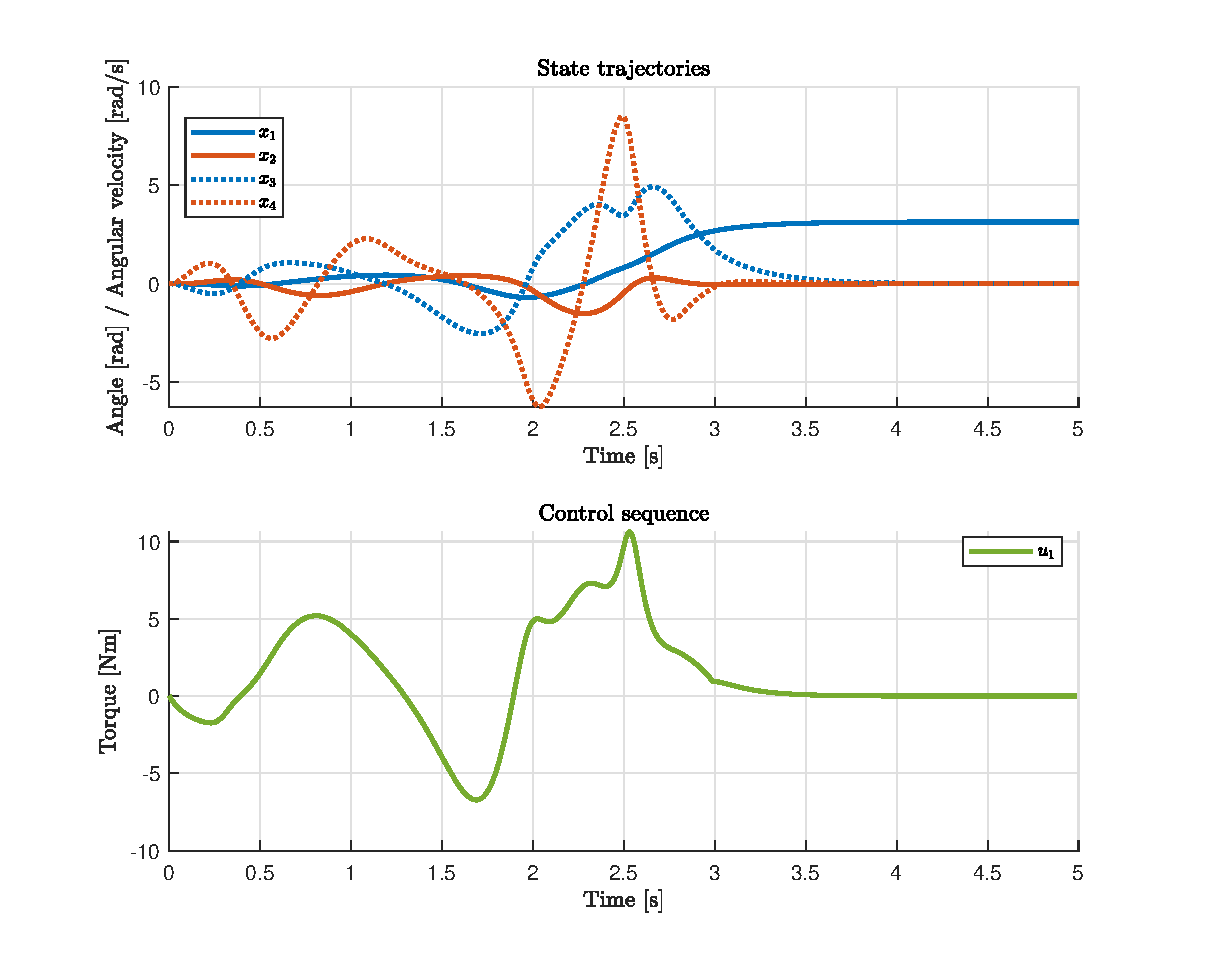
\includegraphics[width=0.4\textwidth]{assets/pendubot_traj.eps}
    \includegraphics[width=0.4\textwidth]{assets/pendubot_nc_traj.eps} \\
    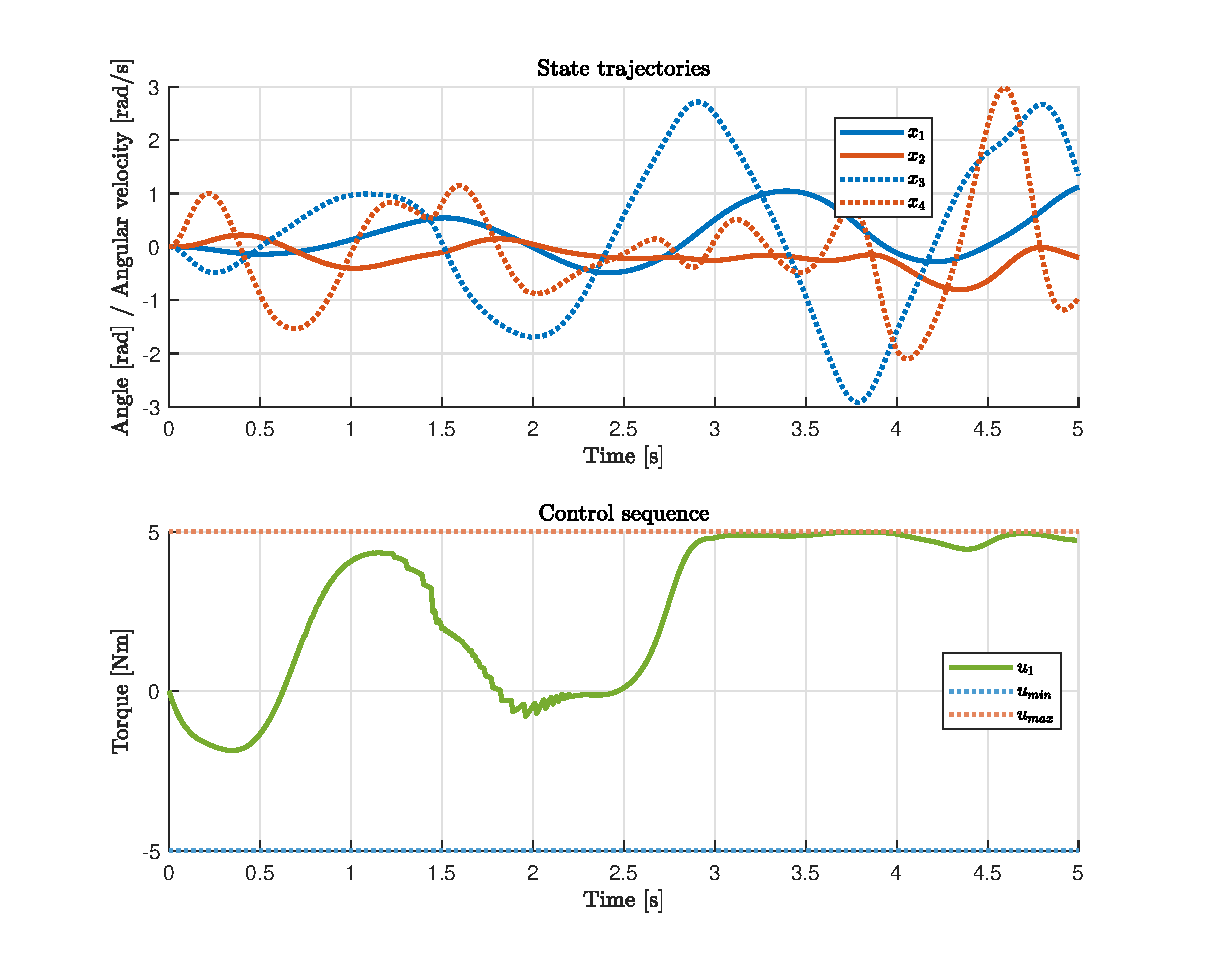
\includegraphics[width=0.4\textwidth]{assets/pendubot_sf_traj.eps}
    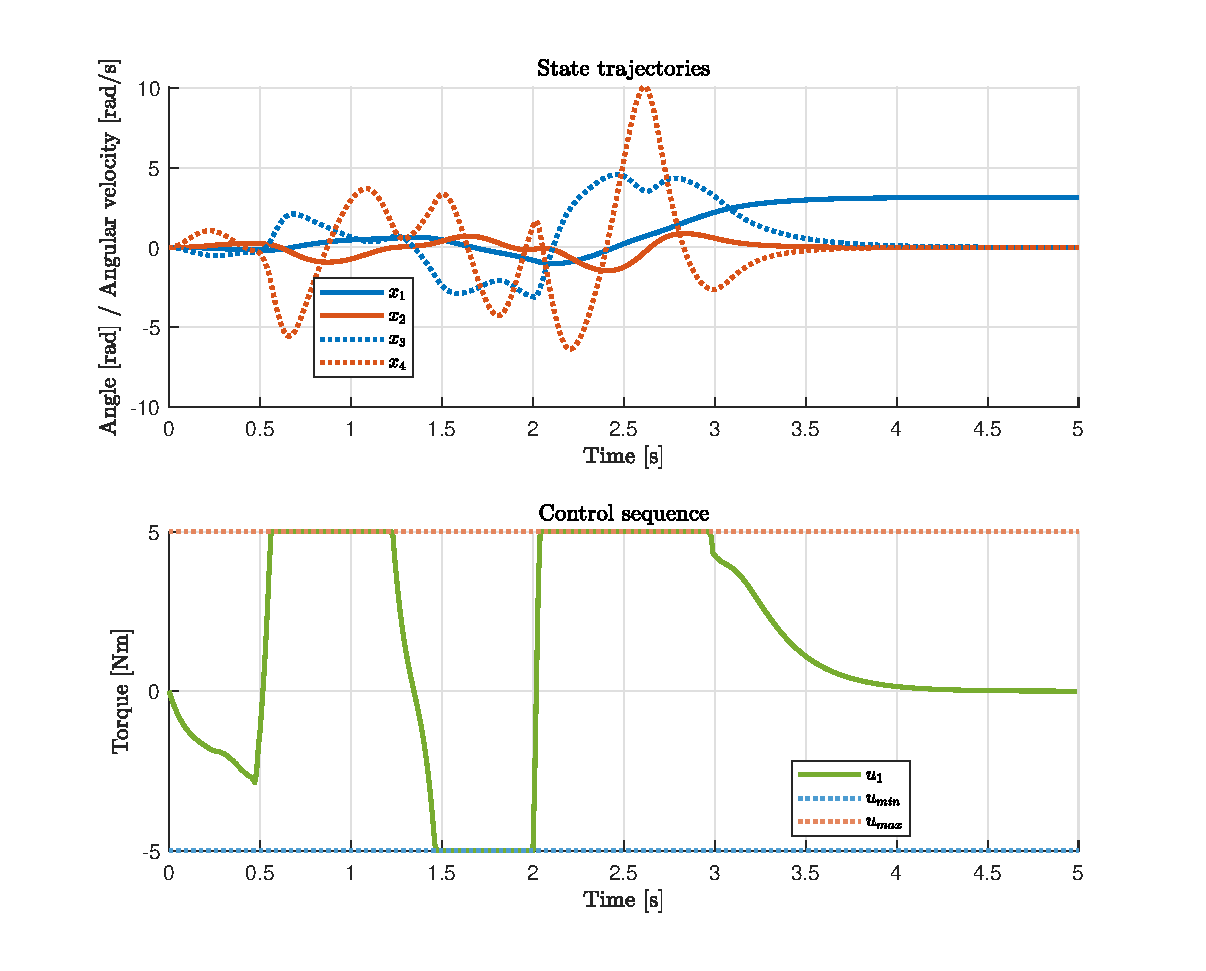
\includegraphics[width=0.4\textwidth]{assets/pendubot_qp_traj.eps}
    \caption{Trajectories of the pendubot under: no constraints (top left), naive clamping (top right), squashing function (bottom left), constrained quadratic programming (bottom right).}
    \label{fig:pendubot_traj}
\end{figure}

\begin{figure}[H]
    \centering
    \includegraphics[width=0.25\textwidth,trim={3cm 1cm 1cm 1cm},clip]{assets/pendubot_qp_anim_1.eps} \hspace*{-0.5cm}
    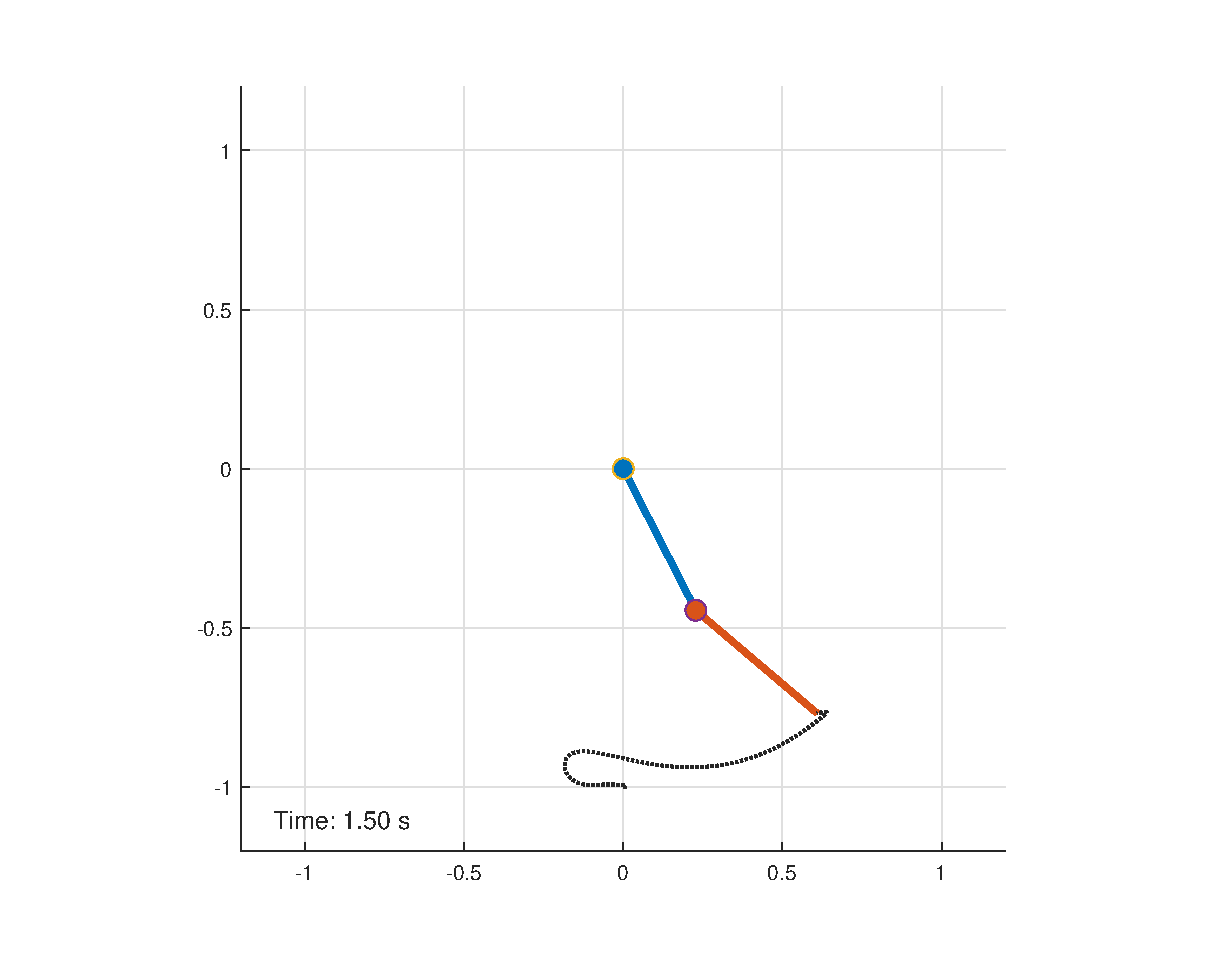
\includegraphics[width=0.25\textwidth,trim={3cm 1cm 1cm 1cm},clip]{assets/pendubot_qp_anim_2.eps} \hspace*{-0.5cm}
    \includegraphics[width=0.25\textwidth,trim={3cm 1cm 1cm 1cm},clip]{assets/pendubot_qp_anim_3.eps} \hspace*{-0.5cm}
    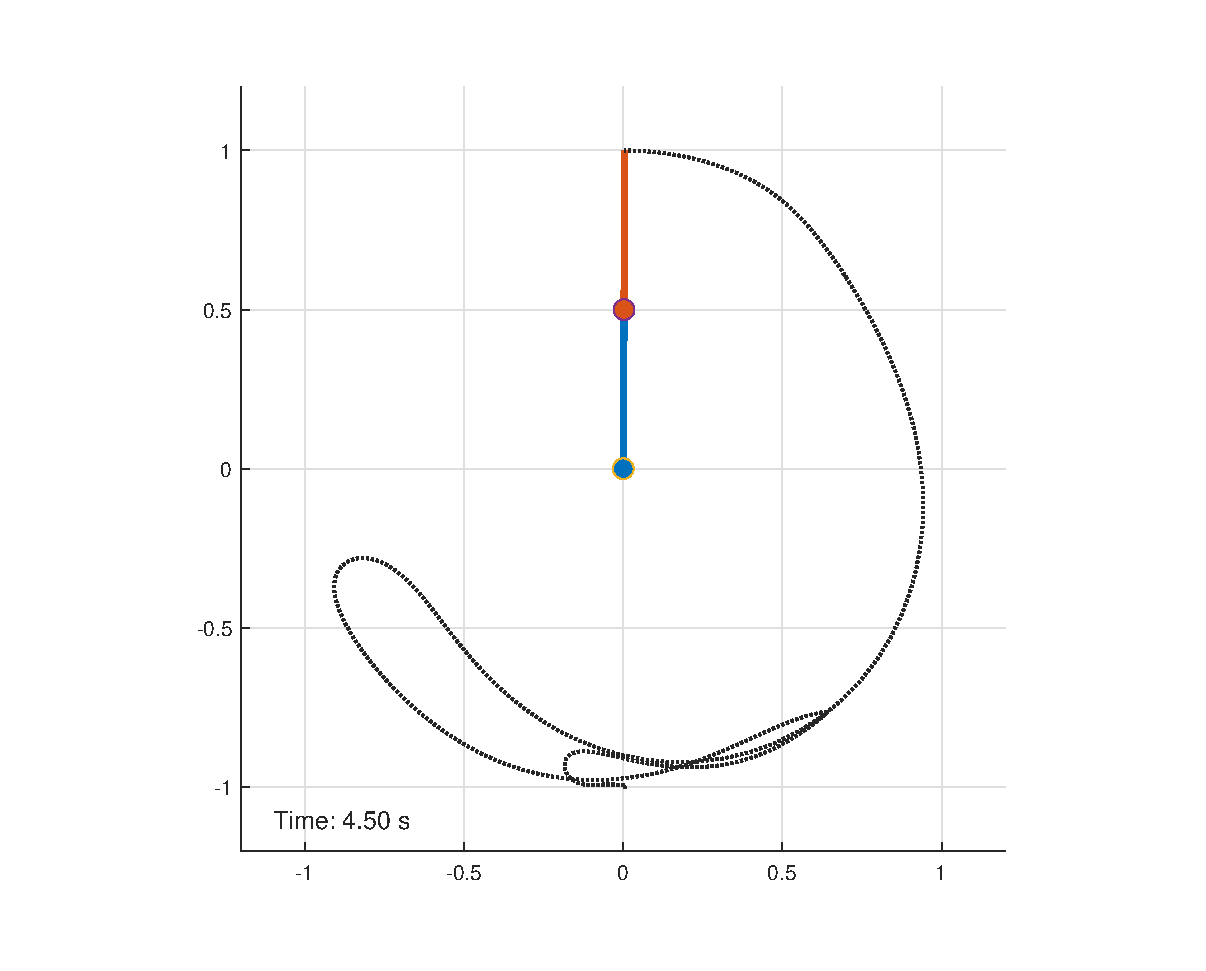
\includegraphics[width=0.25\textwidth,trim={3cm 1cm 1cm 1cm},clip]{assets/pendubot_qp_anim_4.eps}
    \caption{Animation frames of the pendubot swing-up motion under constrained quadratic programming.}
    \label{fig:pendubot_anim}
\end{figure}
\begin{multicols}{2}

\subsubsection{Acrobot}
Conversely, the model of the acrobot is retreived by not actuating the first joint of the robot in Figure \ref{fig:robot}, i.e., by setting $u_1$ identically equal to zero. This time, the limits imposed on the actuated joint are $u_{\text{min}} = -\SI{3.5}{\newton\meter}$ and $u_{\text{max}} = \SI{3.5}{\newton\meter}$, which are less restrictive than the previous case due to the different physical properties of the robot.

Just as it was done for the pendubot, the trajectories of the acrobot under the three different constraining strategies are depicted in Figure \ref{fig:acrobot_traj}, and the animation of the swing-up motion under constrained quadratic programming is shown in Figure \ref{fig:acrobot_anim}. The results are consistent with the previous expreriments, as the constrained quadratic programming method is the only one able to perform the swing-up motion, besides the case with no constraints. In addition to this, note the fact that, when employing naive clamping or the squashing function, the control sequences are similar to each other, are not too close to the extremes of the admissibility interval, and yet are unable to achieve the intended goal: evidently, the constraining methods have penalized the search for the optimal solution during the controller iterations, reflecting the disadvantages that were pointed out in the related section.

\end{multicols}
\begin{figure}[H]
    \centering
    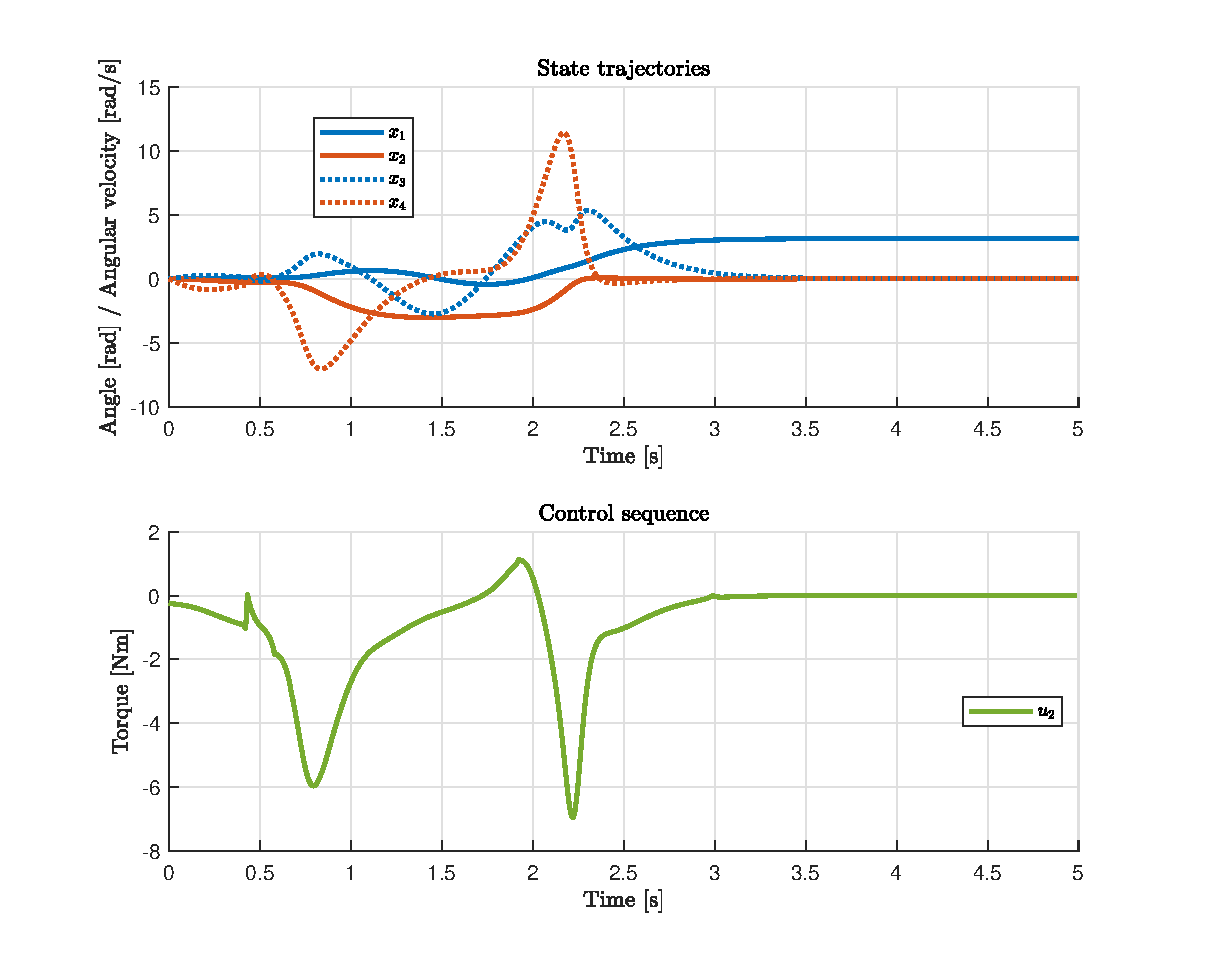
\includegraphics[width=0.4\textwidth]{assets/acrobot_traj.eps}
    \includegraphics[width=0.4\textwidth]{assets/acrobot_nc_traj.eps} \\
    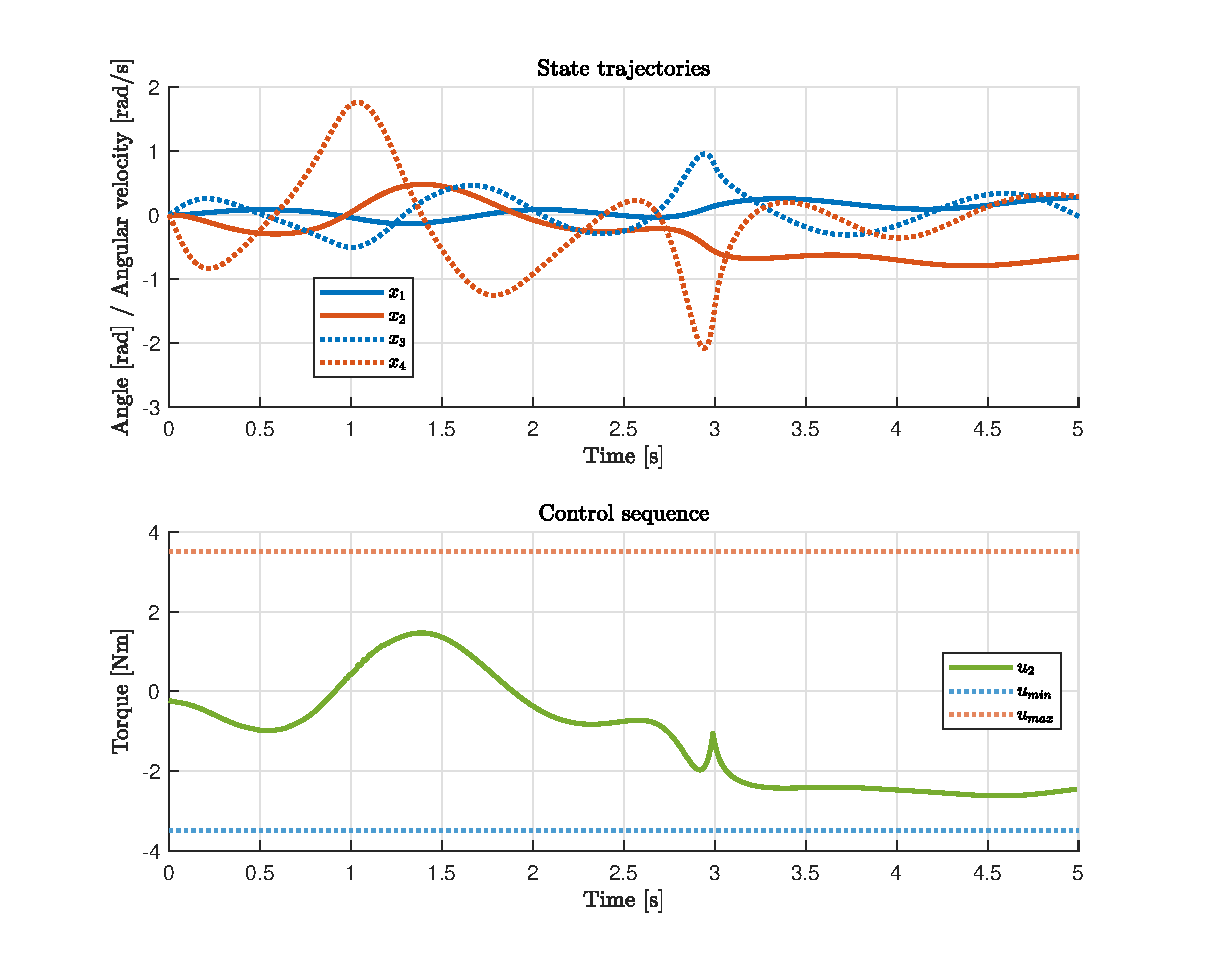
\includegraphics[width=0.4\textwidth]{assets/acrobot_sf_traj.eps}
    \includegraphics[width=0.4\textwidth]{assets/acrobot_qp_traj.eps}
    \caption{Trajectories of the acrobot under: no constraints (top left), naive clamping (top right), squashing function (bottom left), constrained quadratic programming (bottom right).}
    \label{fig:acrobot_traj}
\end{figure}

\begin{figure}[H]
    \centering
    \includegraphics[width=0.25\textwidth,trim={3cm 1cm 1cm 1cm},clip]{assets/acrobot_qp_anim_1.eps} \hspace*{-0.5cm}
    \includegraphics[width=0.25\textwidth,trim={3cm 1cm 1cm 1cm},clip]{assets/acrobot_qp_anim_2.eps} \hspace*{-0.5cm}
    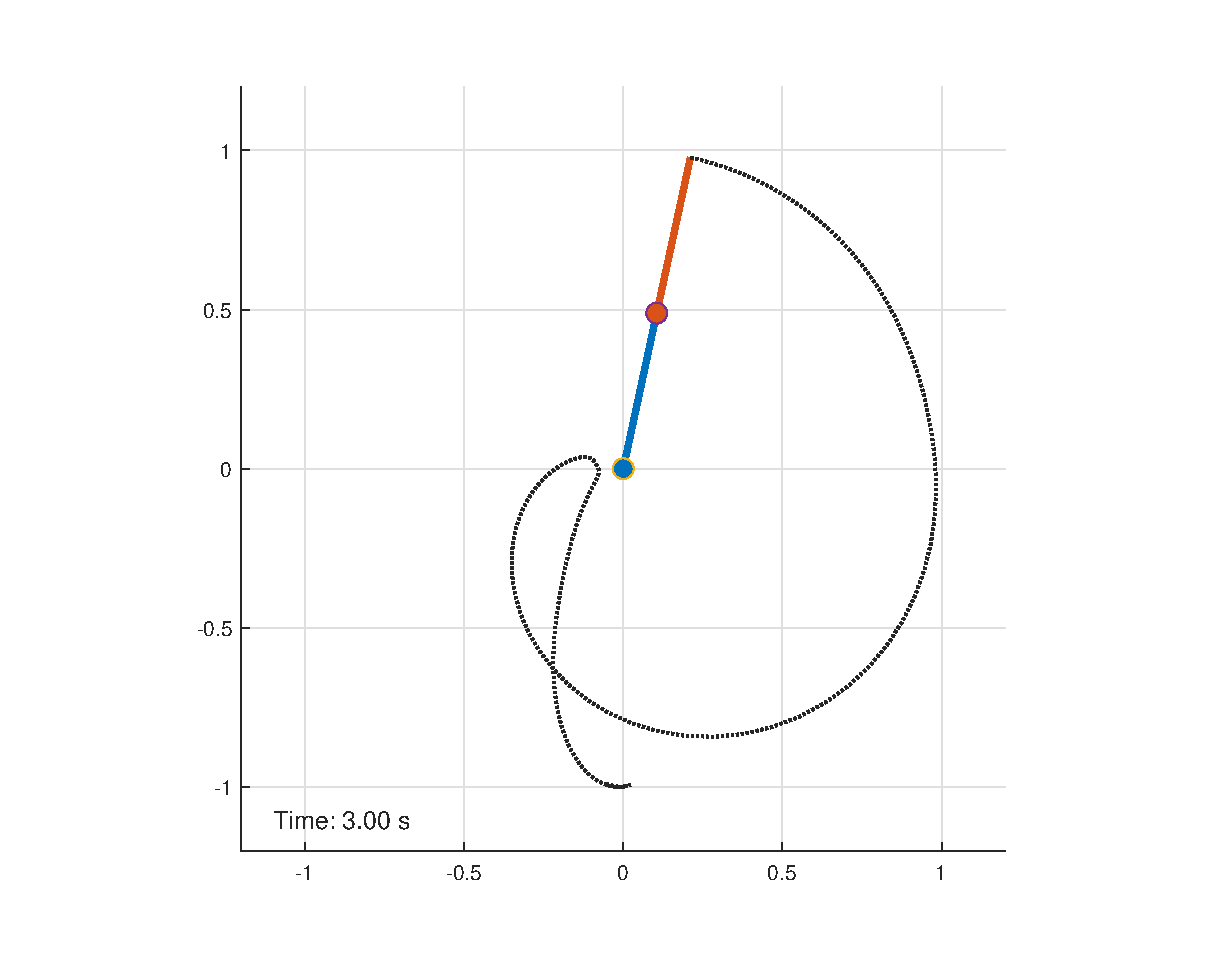
\includegraphics[width=0.25\textwidth,trim={3cm 1cm 1cm 1cm},clip]{assets/acrobot_qp_anim_3.eps} \hspace*{-0.5cm}
    \includegraphics[width=0.25\textwidth,trim={3cm 1cm 1cm 1cm},clip]{assets/acrobot_qp_anim_4.eps}
    \caption{Animation frames of the acrobot swing-up motion under constrained quadratic programming.}
    \label{fig:acrobot_anim}
\end{figure}
\begin{multicols}{2}
        \section{Conclusion}

This paper presents a comprehensive approach to the control of underactuated robots using input-constrained receding-horizon Differential Dynamic Programming. The study focuses on the pendubot and the acrobot, which are exemplary underactuated systems that highlight the challenges and advantages of such control strategies.

The DDP algorithm, renowned for its efficiency in handling nonlinear systems, is adapted to accommodate hard input constraints through three primary methods: naive clamping, squashing functions, and constrained quadratic programming. Among these, the constrained quadratic programming approach proves superior, effectively managing the swing-up problem of both robots while adhering to input constraints. Moreover, the implementation of a receding-horizon strategy, akin to Model Predictive Control, further enhances the real-time applicability of the DDP algorithm. 

Simulation results validated the effectiveness of the proposed method. Whereas naive clamping and squashing functions failed to achieve the desired swing-up motions (because the first method causes a blockage of some search directions, while the second one introduces unrequired and harmful nonlinearities), the constrained quadratic programming method managed to attain the objective, demonstrating both accuracy and efficiency. These simulations not only confirmed the theoretical advantages but also underscored the practical feasibility of the approach. 

In summary, the research illustrates that input-constrained receding-horizon DDP is a robust and efficient method for controlling underactuated robots. It effectively balances the need for constraint satisfaction with the performance demands of nonlinear control tasks. Future work could extend this approach to more complex systems and explore integration with other control methodologies to further improve robustness and adaptability.
        \printbibliography
    \end{multicols}
\end{document}